% !TEX root = DesignDocument.tex

\section{File Conversion Testing}
\tab
    The file conversion is manually tested using a variety of inputs to ensure robust and consistent performance. As there are two libraries (assimp and FBX SDK), they were both manually tested for simple functionality as they were implemented. We tried sending through file types that can be inputs for assimp and made sure that the file made it to the FBX section and output the correct file format (.fbx). There are many different inputs so we sent through files for the common types we would expect such as .stl, .obj, .dae etc. Unsupported file types were also tested and we received appropriate errors from the conversion libraries. The file types supported for our system are available in Table \ref{tab:suportedfiletypes}. We also tried large files so we would know how long we could expect the system to take to process files of different sizes. There are certain limitations on the HoloLens hardware for file size and complexity that can be rendered, so we are aware of the limitations on that end and will inform our users appropriately.\\ 
    
    We also tested files with textures embedded in them, to make sure the textures get converted with the file. With the file types we tried such as .obj and .fbx, the textures converted with the files as expected. The default 3d file viewer in the HoloLens currently does not support colors or textures, so we have not been able to test these features on the HoloLens yet.\\

    The test files we ran through our system came from a variety of sources. We had a simple sphere generated in Maple as a .stl file, which we successfully converted through our system to .fbx to view on the HoloLens. We also received a .fbx representing a column, sent to us from a mathematics professor. The website \url{http://free3d.com} has many 3d files of varying formats and we ran some of them through our system. Sample files included a car, building, space ship, Batman, and other unique files. These files were available as .fbx and were good for testing out the HoloLens, but usually other formats came with them that we could convert them to .fbx as well. Lastly, we received some sample architectural files from one student's family member that were drawings of large buildings in .fbx format. One of these files rendered in the HoloLens, but the other two were too large to render because they exceeded the mesh/vertex limit for the viewer. This was when we looked into the limitations of the built in viewer.\\

    An example of converting a file through our system can be seen below in Figures \ref{Car-FBX}, \ref{Car-OBJ}, and \ref{Car-STL}. 
    We found a 3d file for a car online in the FBX format. 
    Our system then converted it to an OBJ format, as the File Converter software determined it only needed the FBX SDK to convert from FBX $\rightarrow$ OBJ. 
    The third model is an STL file generated from the FBX file, using a DAE file as an intermediate format between the FBX SDK and assimp libraries. 
    As is apparent in Figure \ref{Car-STL} below, the STL file does not contain the colors or smooth surfaces that are present in the other file types, and this is a limitation of the STL file format. 
    This system works for converting STL $\rightarrow$ FBX as well, but the colors would not be present in the final file because that information is not contained in the STL. The STL format is one that can be exported from Maple software.\\

\begin{figure}[H]
    \centering
    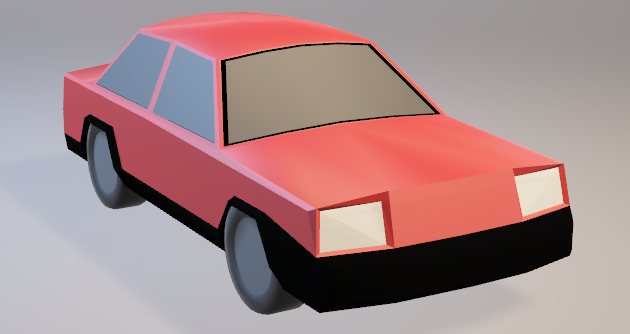
\includegraphics[width=\textwidth]{Car-FBX.png}
    \caption{Car FBX File}
    \label{Car-FBX}
\end{figure}

\begin{figure}[H]
    \centering
    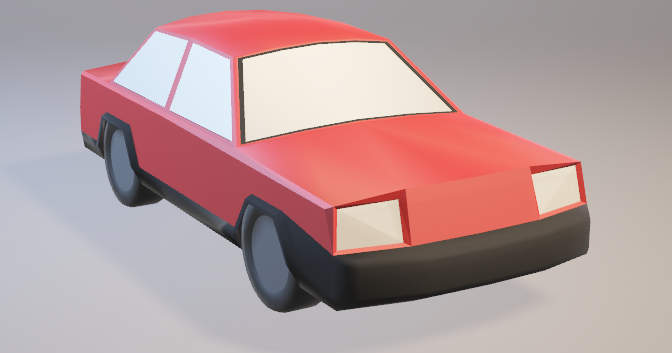
\includegraphics[width=\textwidth]{Car-OBJ.png}
    \caption{Car OBJ File}
    \label{Car-OBJ}
\end{figure}

\begin{figure}[H]
    \centering
    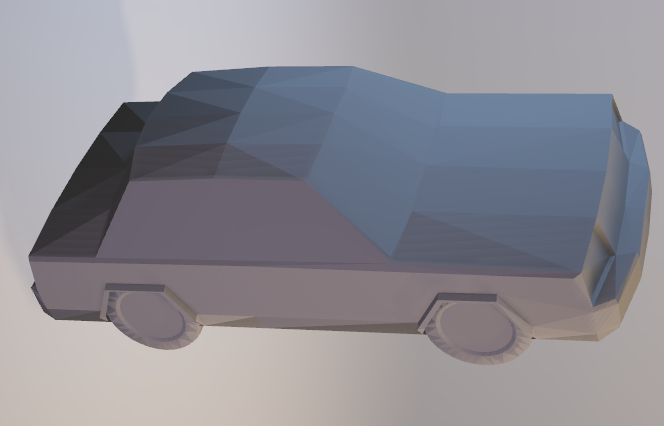
\includegraphics[width=\textwidth]{Car-STL.png}
    \caption{Car STL File}
    \label{Car-STL}
\end{figure}
